\chapter{The Unified Benchmark}

Having validated the harness (Chapter 3), we now place all three
algorithm families on it and establish the thesis's organizing finding.
This chapter reports competitive ratios (mean \(\pm\) 95\% CI) as a
function of prediction quality, in three panels chosen to span the
regimes each family was designed for; the four findings it draws out
(§4.2) recur through the rest of the thesis.

\section{Design}

The families consume different prediction objects, so each is driven by
its own corruption knob and reported in a parallel panel (Chapter 3);
the shared harness (graphs, \(\mathrm{OPT}\), CI methodology, and the
advice-free floor) is what makes the panels comparable.

\textbf{Instance format and notation.} Every panel uses the instance
format of Chapter 3: \(n\) offline resources, \(r\) online request
types, and \(m\) arrivals drawn i.i.d. from the type distribution;
throughout this chapter \(m=n\), so requests and resources are balanced.
The panels differ only in the type graph connecting requests to
resources; that single change is what moves the input between the
regimes the two prediction families were designed for. The three are
chosen so that a degree predictor has strong signal, weak signal, and no
role at all, respectively:

\begin{itemize}
\tightlist
\item
  \textbf{Panel A: heavy-tailed degrees (Zipf)} (\(n=1000\), 60 trials):
  resource degrees follow a Zipf power law with exponent \(1.0\), so a
  few resources are heavily contended while most are rarely eligible.
  This heavy-tailed profile gives a degree predictor genuine signal to
  carry.
\item
  \textbf{Panel B: left-regular \(d{=}5\)} (\(n=1000\), 60 trials): each
  arriving request connects to exactly \(d=5\) uniformly random
  resources, so resource degrees are nearly homogeneous: the hard case
  of Chapter 3, where a degree predictor has almost no signal left to
  carry.
\item
  \textbf{Panel C: few-types \(r{=}8\)} (\(n=2000\), 50 trials): only
  \(r=8\) distinct request types, each arriving \(\approx n/r=250\)
  times on average: the near-perfect-matchable, few-types regime the
  histogram-advice algorithms are calibrated for; their
  test-and-fallback test inspects a prefix of \(k=200\) arrivals.
\end{itemize}

Panels A and B thus exercise the degree-prediction family (MPD and its
augmentations); Panel C exercises the histogram-advice family
(FollowPrediction, TestAndMatch, and the combiner).

\textbf{Shared methodology.} Paired trials, independent random streams
and confidence intervals are exactly as in §3.5; the panel-specific
parameters are the ones listed above, and the intervals are tight
throughout (\(\pm0.001\)--\(0.003\)). The quality columns instantiate
the error models of §3.3. Degree panels: \emph{perfect} (true realized
degrees), \emph{noisy} (random-flip at strength \(\tfrac12\)),
\emph{adversarial} (order-reversing reflection), \emph{garbage}
(independent random \(\mu\), \(\equiv\) Ranking); advice panel: the true
histogram blended toward a concentrated random target by
\(\eta\in\{0,0.3,0.6,1.0\}\) (\emph{perfect / mild / bad / garbage}).
The two sets of columns are not commensurable (they corrupt different
prediction objects with different knobs), so only within-panel
comparisons carry meaning. \textbf{Table 4.1} presents each panel's
ratios beside its bar chart; the findings follow in §4.2.

\begin{table}[H]
\footnotesize
\setlength{\tabcolsep}{4pt}
\noindent
\begin{minipage}[c]{0.60\linewidth}
\begin{tabular}{@{}lrrrr@{}}
\toprule
\emph{Panel A --- heavy-tailed (Zipf)} & perfect & noisy & advers. & garbage \\
\midrule
Ranking (floor) & 0.948 & --- & --- & --- \\
MinDegree (oracle) & 0.996 & --- & --- & --- \\
MPD & 0.989 & 0.956 & \textbf{0.908} & 0.946 \\
Feldman(MPD) & 0.981 & 0.979 & 0.976 & 0.978 \\
JailletLu(MPD) & 0.977 & 0.976 & 0.974 & 0.975 \\
Feldman (base) & 0.887 & --- & --- & --- \\
JailletLu (base) & 0.900 & --- & --- & --- \\
\bottomrule
\end{tabular}
\end{minipage}\hfill
\begin{minipage}[c]{0.38\linewidth}
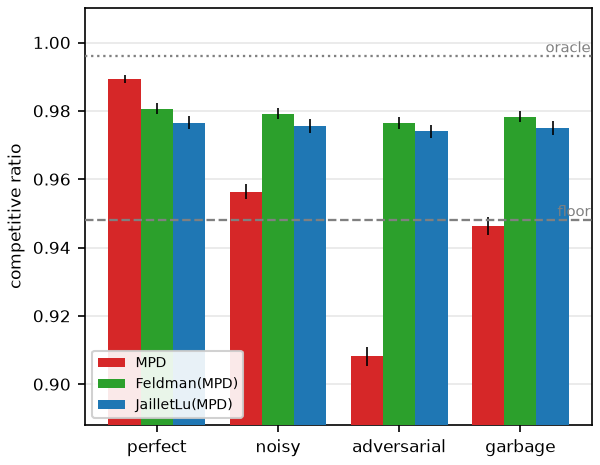
\includegraphics[width=\linewidth]{../../results/unified_benchmark_panelA.png}
\end{minipage}

\medskip
\noindent
\begin{minipage}[c]{0.60\linewidth}
\begin{tabular}{@{}lrrrr@{}}
\toprule
\emph{Panel B --- left-regular $d{=}5$} & perfect & noisy & advers. & garbage \\
\midrule
Greedy $=$ Ranking (floor) & 0.890 & --- & --- & --- \\
MinDegree (oracle) & 0.966 & --- & --- & --- \\
MPD & 0.932 & 0.906 & \textbf{0.854} & 0.888 \\
Feldman(MPD) & 0.906 & 0.902 & 0.896 & 0.900 \\
JailletLu(MPD) & 0.904 & 0.903 & 0.899 & 0.901 \\
Feldman (base) & 0.760 & --- & --- & --- \\
JailletLu (base) & 0.788 & --- & --- & --- \\
\bottomrule
\end{tabular}
\end{minipage}\hfill
\begin{minipage}[c]{0.38\linewidth}
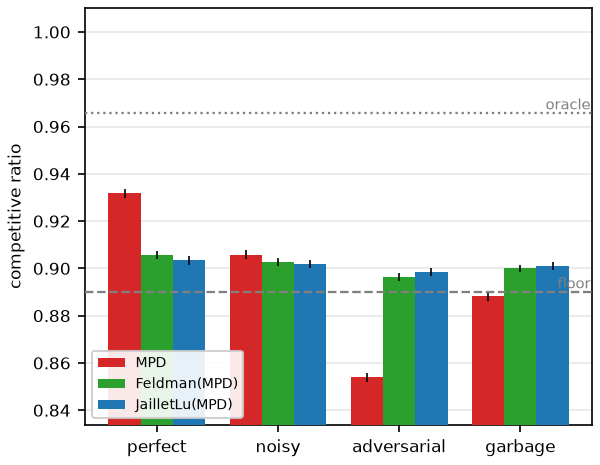
\includegraphics[width=\linewidth]{../../results/unified_benchmark_panelB.png}
\end{minipage}

\medskip
\noindent
\begin{minipage}[c]{0.60\linewidth}
\begin{tabular}{@{}lrrrr@{}}
\toprule
\emph{Panel C --- few-types $r{=}8$} & perfect & mild & bad & garbage \\
\midrule
Ranking (floor) & 0.990 & --- & --- & --- \\
MinDegree (oracle) & 0.999 & --- & --- & --- \\
FollowPrediction & 1.000 & 0.832 & 0.679 & \textbf{0.472} \\
TestAndMatch (Choo) & 1.000 & 0.984 & 0.989 & 0.990 \\
TestAndMatch (BEM) & 0.998 & 0.988 & 0.988 & 0.968 \\
Combiner \emph{(benchmark)} & 0.990 & 0.990 & 0.990 & 0.990 \\
\bottomrule
\end{tabular}
\end{minipage}\hfill
\begin{minipage}[c]{0.38\linewidth}
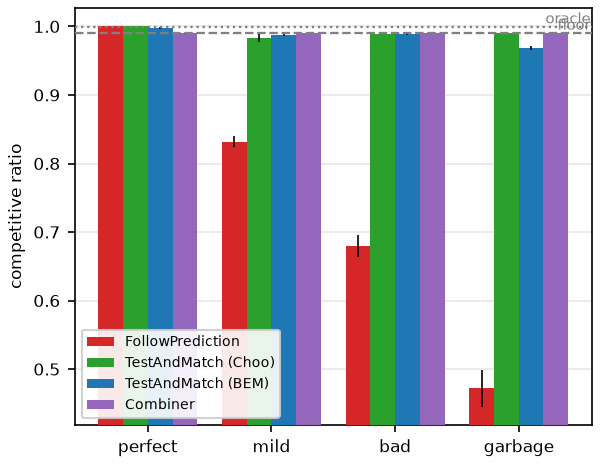
\includegraphics[width=\linewidth]{../../results/unified_benchmark_panelC.png}
\end{minipage}
\caption{The unified benchmark. Each panel's competitive ratios (means over paired
trials; every 95\% CI $\le 0.003$) sit beside their bar chart (error bars: 95\% CIs;
dashed line: advice-free floor; dotted: oracle ceiling). Bold marks the worst column of
each unguarded prediction-follower; all three fall below their own panel's floor. That
floor is instance-dependent --- it is Ranking's ratio on that panel's graph family, not a
constant --- so the three floors ($0.948$, $0.890$, $0.990$) are not comparable with one
another, and neither are the quality columns across the two prediction families (\S3.3).}
\end{table}

\section{Four findings}

\textbf{(F1) Robustness is engineered, not free: naive followers crash
below the floor.} Both unguarded prediction-followers dive under the
advice-free Ranking floor once the prediction is adversarial or garbage:
MPD falls to \(0.908<0.948\) (Panel A) and \(0.854<0.890\) (Panel B),
and FollowPrediction collapses to \(0.472\ll0.990\) (Panel C). Under
adversarial or garbage advice, then, using either \emph{unguarded} is
worse than using no prediction at all. Every robust algorithm (the
augmentations, TestAndMatch, the combiner) avoids this by construction.

\textbf{(F2) Two distinct robustness mechanisms, with different shapes.}
\emph{Structural} robustness (Feldman(MPD), JailletLu(MPD)): the
worst-case-optimal base matching carries the load and the prediction
only breaks ties, so performance is nearly flat: Feldman(MPD) moves only
\(0.981\!\to\!0.976\) from perfect to adversarial (Panel A). It cannot
crash but caps the upside (never reaching the \(0.996\) oracle).
\emph{Adaptive} robustness (TestAndMatch): test a sublinear prefix, then
commit, capturing the upside when advice is good (Choo \(1.000\)) and
holding the floor when it is bad (\(0.990\)). On Panel C it is the only
algorithm on the upper envelope at both ends. The two mechanisms trade
consistency for robustness in opposite ways; \textbf{Figure 4.1} plots
every algorithm on the consistency--robustness plane, where the opposite
trades, and the empty region beyond TestAndMatch toward the ideal
top-right corner, are visible at a glance.

\begin{figure}
\centering
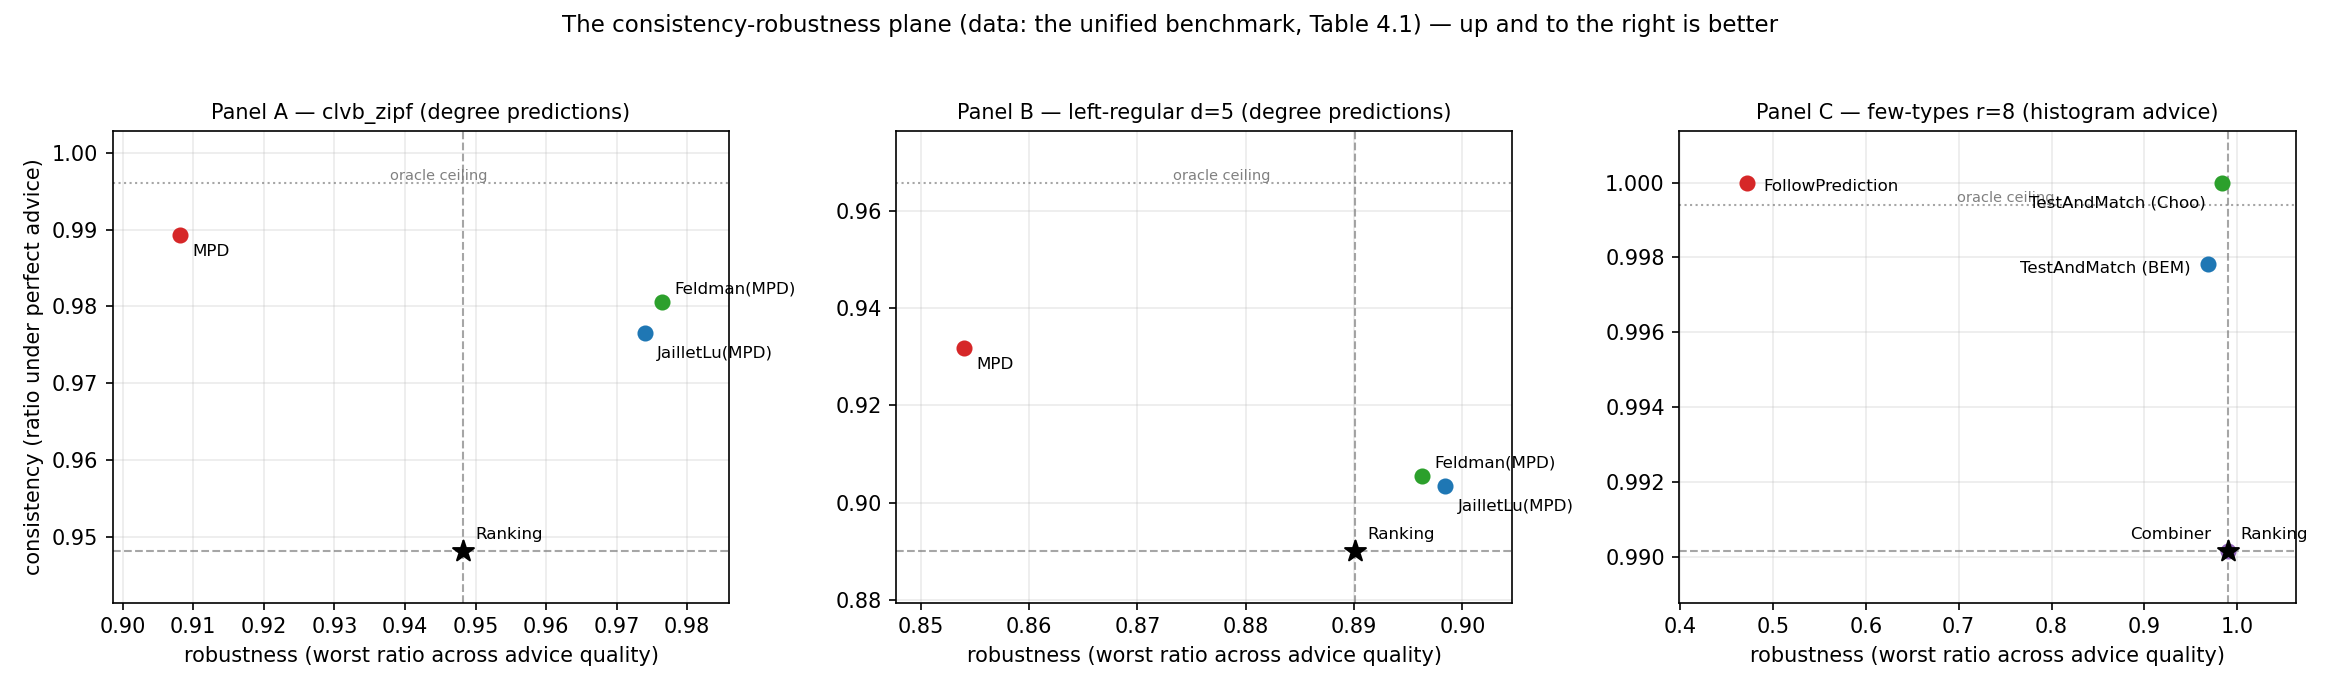
\includegraphics[width=1\linewidth,height=\textheight,keepaspectratio,alt={The consistency--robustness plane (the data of Table 4.1). Horizontal axis: ratio under perfect advice. Vertical axis: ratio under the worst corruption level, the operational robustness of §3.4. Dashed lines mark the advice-free floor, dotted the oracle ceiling; TestAndMatch sits nearest the ideal top-right corner.}]{../../results/consistency_robustness.png}
\caption{The consistency--robustness plane (the data of Table 4.1).
Horizontal axis: ratio under perfect advice. Vertical axis: ratio under
the worst corruption level, the operational robustness of §3.4. Dashed
lines mark the advice-free floor, dotted the oracle ceiling;
TestAndMatch sits nearest the ideal top-right corner.}
\end{figure}

\textbf{(F3) The consistency upside is small on average-case inputs; the
spread lives on the bad-advice side.} On few-types the advice-free
Ranking is already \(0.990\) and MPD-with-true-degrees is \(0.999\): the
entire consistency headroom is \(0.009\pm0.001\), smaller than most of
the effects measured later in this thesis. Every wide gap in Panel C is
a \emph{downside} gap. This is the thesis in one panel; Chapter 6 shows
why no affordable test escapes it, and the concluding outlook (§10.2)
why it is forced.

\textbf{(F4) The augmentation rescues structurally weak base
algorithms.} Feldman and Jaillet--Lu are tuned for the worst-case ratio
and are the weakest advice-free entries on these average-case inputs
(Panel B: \(0.760\) / \(0.788\), below Greedy's \(0.890\)); the MPD
augmentation lifts them to \(\approx0.90\). The prediction does more for
the worst-case-designed algorithms than for greedy, a pairing that a
unified table makes immediate.

\section{Chapter summary}

The value of a prediction here is downside protection, not performance.
The next question is what governs the loss that remains, and Chapter 5
shows it is not the size of the prediction error but the order it
induces.
